\documentclass{sig-alternate}
\usepackage{algorithm}
\usepackage{algorithmic}
\usepackage{url}
\usepackage{subfigure}

\begin{document}

\title{Crowdy: Social Crowd Visualization}

\numberofauthors{1} 
\author{\alignauthor Jeffrey McGee, Zhiyuan Cheng, Chiao-Fang Hsu, Pratheek Kumar Akireddy \\
\affaddr{Department of Computer Science and Engineering, Texas A\&M University} \\ \affaddr{ College Station, TX 77845 USA} \\
\email{jeffamcgee@gmail.com, chengzhy@gmail.com, drakihsu@cse.tamu.edu, pka293@cse.tamu.edu}
} 

\maketitle
\begin{abstract}
Microblogging systems has provided the society with a more transparent channel for information distribution. Each individuals are empowered to spread the news and build their social networks. With the freedom of information generation, the issue now is the ``useful information'' identification, organization and visualization. For this project, we want to design an user interface that take both usefulness and usability into consideration. Our system will be able to adapt to different types of user and display the crowds emerged in a specific period of time as well as the topics discussed by the crowd from Twitter. The interface should both optimize the user experience and system speed. For evaluation, we will design some user study or inspection procedures in order to test the efficiency, effectivness and satisfaction of this system to our poential users.
\end{abstract}

\category{H.5.1}{Information Interfaces and Presentation}{Multimedia
Information Systems}[video]
\category{H.5.3}{Group and Organization Interfaces}[collaborative computing, computer-supported cooperative work]
\category{H.5.4}{Hypertext/Hypermedia}[architecture]

\terms{Design, Experimentation, Human Factors}

\keywords{interface, crowd, twitter}

\section{Introduction}
Along with the rise of real-time social web, the power of information distribution is no longer limited to the small set of news media but the massive amount of ordinary individuals. Websites like Digg and Reddit provides a news aggregation platform that filter and display interesting news pieces recommended by other users; social media object sharing sites like Youtube and Flickr let users to upload and browse videos and images; microblogging systems, like Twitter and Buzz, enable every user to host a broadcasting station of their own; last but not least, Facebook with all the mentioned function available, allowing users to build their own online social network and share their everyday experience with their friends. Thus, the need for services that exploit these massive data is increasing. People are looking for a new generation of applications for monitoring, analyzing, and distilling information from the prospective web of real-time content that reflects the current activity of the web's participants. The shift toward fresh web content can be seen in the growing interest in mining large-scale social media for information discovery and brand management, for intelligence analysis by the government and state media, and in identifying and disseminating disaster and emergency-related information.

Comparing with the traditional web information applications that apply expensive off-line analysis of web data, the new generation of real-time web applications must be able to consume, process and display the massive amounts of data on-the-fly. In this project, we look particular into twitter, a microblogging system, platform. We want to provide users a manageable exploratory interface that display the crowds and their associated participants/content at each time period. The term ``Crowd'' refers to the emerging hotspots on the real-time web. Unlike long-lived communities or groups, a crowd is intended to reflect a potentially short-lived ad-hoc collection of users. In twitter, there are potentially 100s of millions of active users inserting new messages into the system at a high-rate. With existing algorithm and architecture built by our lab in the backend, our goal is to reveal the ad-hoc crowds of users that reflect the real-time interests and highly-temporal group affiliations in a clear and manageable fashion.

Even though our current data is from Twitter, we expect the system to be useful to users who are not familiar with twitter. In fact, our system can be of useful to several types of users with different purpose in mind.

\subsubsection{How Might We Help}
Apart from the original twitter interface that provides only a local view of the most current tweets issued by each user's followee or some local trending topics, our final system should be able to aggregate the data to find global, regional, and local phenomenons. The final product is also adjustable that fit into different expertise and purpose of usage based on the role of the users.

\subsection{Conceptual Model}
The conceptual model of our system is a tool for finding patterns, trends, and communities. The interface displays groups of people who are talking with each other, puts their conversation on a map, and finds important words in the conversation. Users will expect different types of filtering option such as filtering by area(geo-feature), by time(timeline snapshot), by keyword(free-text, hashtag) or by the expecting property of the crowds(the longest living crowd, the most engaging crowd). The default view of the system is a set of global crowd discovered recently.


\subsection{User}
To better design our system interface, we want to understand our potential users. For different kinds of users, there exhibits different patterns of properties like the frequency of usage, the level of experience, the behavior tendency and the tuning options availability.
\begin{itemize}
	\item Analyst: Government or media analyst are experts in information trending and market research. They use the system regularly with the frequency between once per day to once per month depending on the urgency of the monitoring task itself. They would like to have customized interface that is able to make variety of filtering on the fly. They will most likely mine the data using our system and edit the report at the same time.
	
	\item Twitter Users: Twitter users who is already have familiarity with the Twitter world could have interest in using our system to know about crowds and hot-topics. The may use it regularly or occasionally. They adopt our system to assist their twittering experience. They might not devote a big amount of time and effort but just want a quick and fresh view of the current trend. For this purpose, we should provide a simple and personalized content display with some easy filtering options.
	
	\item Regular People: regular users with no Twitter experience would use our system as a window to gain some quick idea to what happened currently in the Twitter world. To satisfy their curiosity without personalized history to learn from, we provide a global trend as the first look. Ideally, the users will come back and build a history profile so we can customize the display in a long run. people could use it just once or , if they like the system, several times per day.
	
	\item Business People - corporate people is particularly interested in their own product or company. Like the analysts, they are asked to perform the trending survey in a regular basis. They are trained in finding information related to their product. They use our system to find the opinion from the general users. They also study their competitors in a hope to improve their own. For this type of user, we can do highly customized interface to pre-filter the crowds to display. We may also prepare a set of template so the business people with no computer science knowledge can easily drag-and-drop views related to their competitors and their own side by side.
	
\end{itemize}

\subsection{Cognitive Issue}
Some cognitive issues we need to consider including the other activities our users might be engaging in simultaneously. For example, the twitter user might be browsing twitter and plan to use our system to understand the crowds that talk about a certain keyword of interest. Another situation can be finding some interesting topics while playing with our system and decide to do search to read the related news article from Google or NY Times. Or, our users may discover an exciting crowd/topic and eager to share this discovery to his friends on the social websites(Twitter, Facebook, etc). That is to say, we does not expect our user to keep 100\% focus on interacting with the system. We need to provide mechanisms for tip reminding of behavior history. 

In addition, with the nature of the temporal massive data, we do not expect our users to remember where to find the crowd/topic of interest that the user just encountered. We want to provide a Workspace panel so to release the stress on the memory requirment from the user.

\section{Related Work}

\section{Interface Design}

\begin{figure*}[t]
\centering
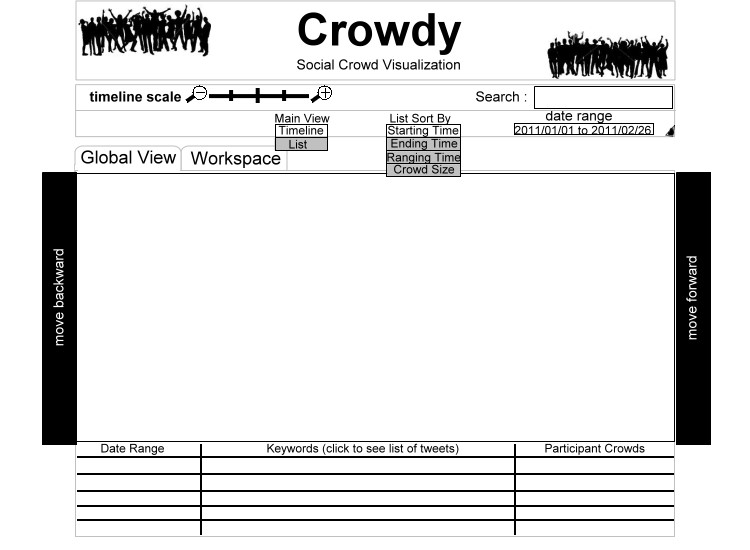
\includegraphics[width=400pt]{img/UIdesign.eps}
\caption{Crowdy User Interface Design}
\label{fig:UIdesign}
\end{figure*}

Figure \ref{fig:UIdesign} shows an outline of the prototype. We want to provide the user with a simple and flexible interface to maximize the exploring experience while minimize the memorizing overhead. Existing web applications show that the most general task should be the main focus and the other available options may be placed on the side or hidden according to their frequency of usage. Recall the primary function of our system is to visualize the Crowds emerged over time, thus, the crowd displaying window comes as our first priority panel for displaying. In the crowd displaying window, we further consider the needs of personalization for our potential users(e.g. Analyst). There is a Global View Panel and a personal workspace panel. The Personal Workspace Panel distinguishes from the Global View Panel in a way that it only shows the set of crowds marked by the user when exploring in the Global View Panel. To help our users quickly and easily transit between these two views, tabbing function is used. Inside each view, we need to decide the format of showing massive amount of timestamp attached crowds which has several metadata associated with it such as starting/ending time, crowd participants, tweets, location data, etc. To effectively organize these properties to assist quick and convenient retrieval by the user, we consider these two formats: timeline and list. For both view panel, these two formats are included but sized unequally. The size is adjustable(in the option panel) according to the user's need. Generally, ``timeline'' is more suitable for overview a larger amount of data while ``list'' is better for detail skimming in a smaller crowd set. We also provide several filtering option for both timeline and list format in the option panel. Some detail component in these three panel are list below.

\begin{itemize}
	\item \textit{Global View Panel} : The global view shows the global crowds in different format. When a crowded is marked by the user, a flag will be placed in front of each crowd item in each format.
			
			\begin{itemize}
				\item Timeline format displays the evolution of each crowd. First of all, a crowd is shown as a line from the starting time to the ending time. The size of the participants over time is indicated by color(e.g., small-large-medium $\longrightarrow$ green-red-blue). Top three keywords that describe the topic of the crowd is displayed explicitly on the timeline along with the crowd line. Extra information about the crowd can be viewed in the pop up box when the user clicks on the crowd line.
				\item List format displays each crowd with some specific sorting order. The default sorting order is by the starting time. Some other available sorting function including the ending time, the size of crowds and the ranging time. In the list format, crowds are displayed explicitly in three columns: time period, keywords and some of the participants. The latter two columns are clickable. After clicked, it will show the list of tweets and the full set of participants in a pop up window form. 
		\end{itemize}			
	
	\item \textit{Personal Workspace Panel} : Similar as the Global View Panel but with only the set of crowds marked by the user in the Global View Panel.
	\item \textit{Filter Option Panel} : This panel explicitly display a set of most frequent used filtering options such as search and timeline scaling bar. We also provide the user with flexibility to adjust the default settings we provided such as the primary displaying format in the View Panel, list sorting function and time period filtering. Other filtering option is hidden and can be expanded when click on the right bottom corner of the Panel.
\end{itemize}

\section{Implementation}

\section{Evaluation}

\section{CONCLUSIONS}

\section{FUTURE WORK}

\bibliographystyle{abbrv}
\bibliography{reference} 
\end{document}